\documentclass[a4paper,fleqn,usenatbib,useAMS]{mnras}

\usepackage{graphicx}	% Including figure files
\usepackage{amsmath}	% Advanced maths commands
\usepackage{amssymb}	% Extra maths symbols
\usepackage{multicol}        % Multi-column entries in tables
\usepackage{bm}		% Bold maths symbols, including upright Greek
\usepackage{pdflscape}	% Landscape pages

\newcommand{\numax}{\ensuremath{\nu_{\textrm{max}}}}
\newcommand{\dnu}{\ensuremath{\Delta\nu}}
\newcommand{\teff}{\ensuremath{T_{\textrm{eff}}}} 
\newcommand{\kep}{\ensuremath{Kepler}}

\newcommand{\bibtex}{\textsc{Bib}\!\TeX} % bibtex. Not quite the correct typesetting, but close enough

\usepackage[T1]{fontenc}
\usepackage{ae,aecompl}
\usepackage{newtxtext,newtxmath}

\title[TRG]{TESS Asteroseismic Predictions for Red Giants using Kepler data}

\author[Mat Schofield]{Mat Schofield$^{1}$\thanks{Contact e-mail: \href{mailto:mxs191@bham.ac.uk}{mxs191@bham.ac.uk}}\thanks{Present address: Department of Physics and Astronomy, the University of Birmingham, Birmingham B15 2TT, UK}
\author[Guy Davies]{Guy Davies}
\\
% List of institutions
$^{1}$Department of Physics and Astronomy, the University of Birmingham, Birmingham B15 2TT, UK}


\date{Last updated 2017 May 31; in original form 2017 May 31}
\pubyear{2015}

\begin{document}
\label{firstpage}
\pagerange{\pageref{firstpage}--\pageref{lastpage}}
\maketitle

\begin{abstract}
{\it Summary}: This paper presents a method to predict Red Giant mode detectability with TESS, using Kernel Density Estimation. It requires only the global parameters \dnu, \numax, the stellar magnitude and length of observation. \newline
{\it Method}: Lightcurves for \kep \ stars with fitted radial mode frequencies were used to generate equivalent TESS lightcurves. The lightcurves were cut down, \kep \ white noise was removed, the bandpass was adjusted, and TESS white noise was added. A detection test was run on the observed modes in these 'TESS-like' lightcurves. Kernel density estimation was then used to determine mode detectability with TESS based upon the global asteroseismic parameters \numax \ and \dnu, as well as the stellar magnitude.\newline
{\it Application}: The method has been designed to be used to make predictions for other missions such as K2, PLATO and CoRoT. The only difference when applying the method for other missions is to adjust the lightcurve transformation.
\end{abstract}


\section{Introduction}


\section{Transforming the lightcurves}

The timeseries data from \kep \ observations needed to be adjusted for a different satellite and mission. This could either be done in the time or frequency domain. Both methods were tested and compared. The time domain method was chosen to transform the lightcurves, and was used in the rest of this work.

Several different adjustments needed to be made to the \kep \ data. One difference between the missions is the length of observation. The \kep \ mission ovserved for 4 years, while TESS' nominal 2 year mission will observe stars for between 27 days to 1 year, according to the star's ecliptic latitude (Figure \ref{TESS field}).

\begin{figure}
	\centering
	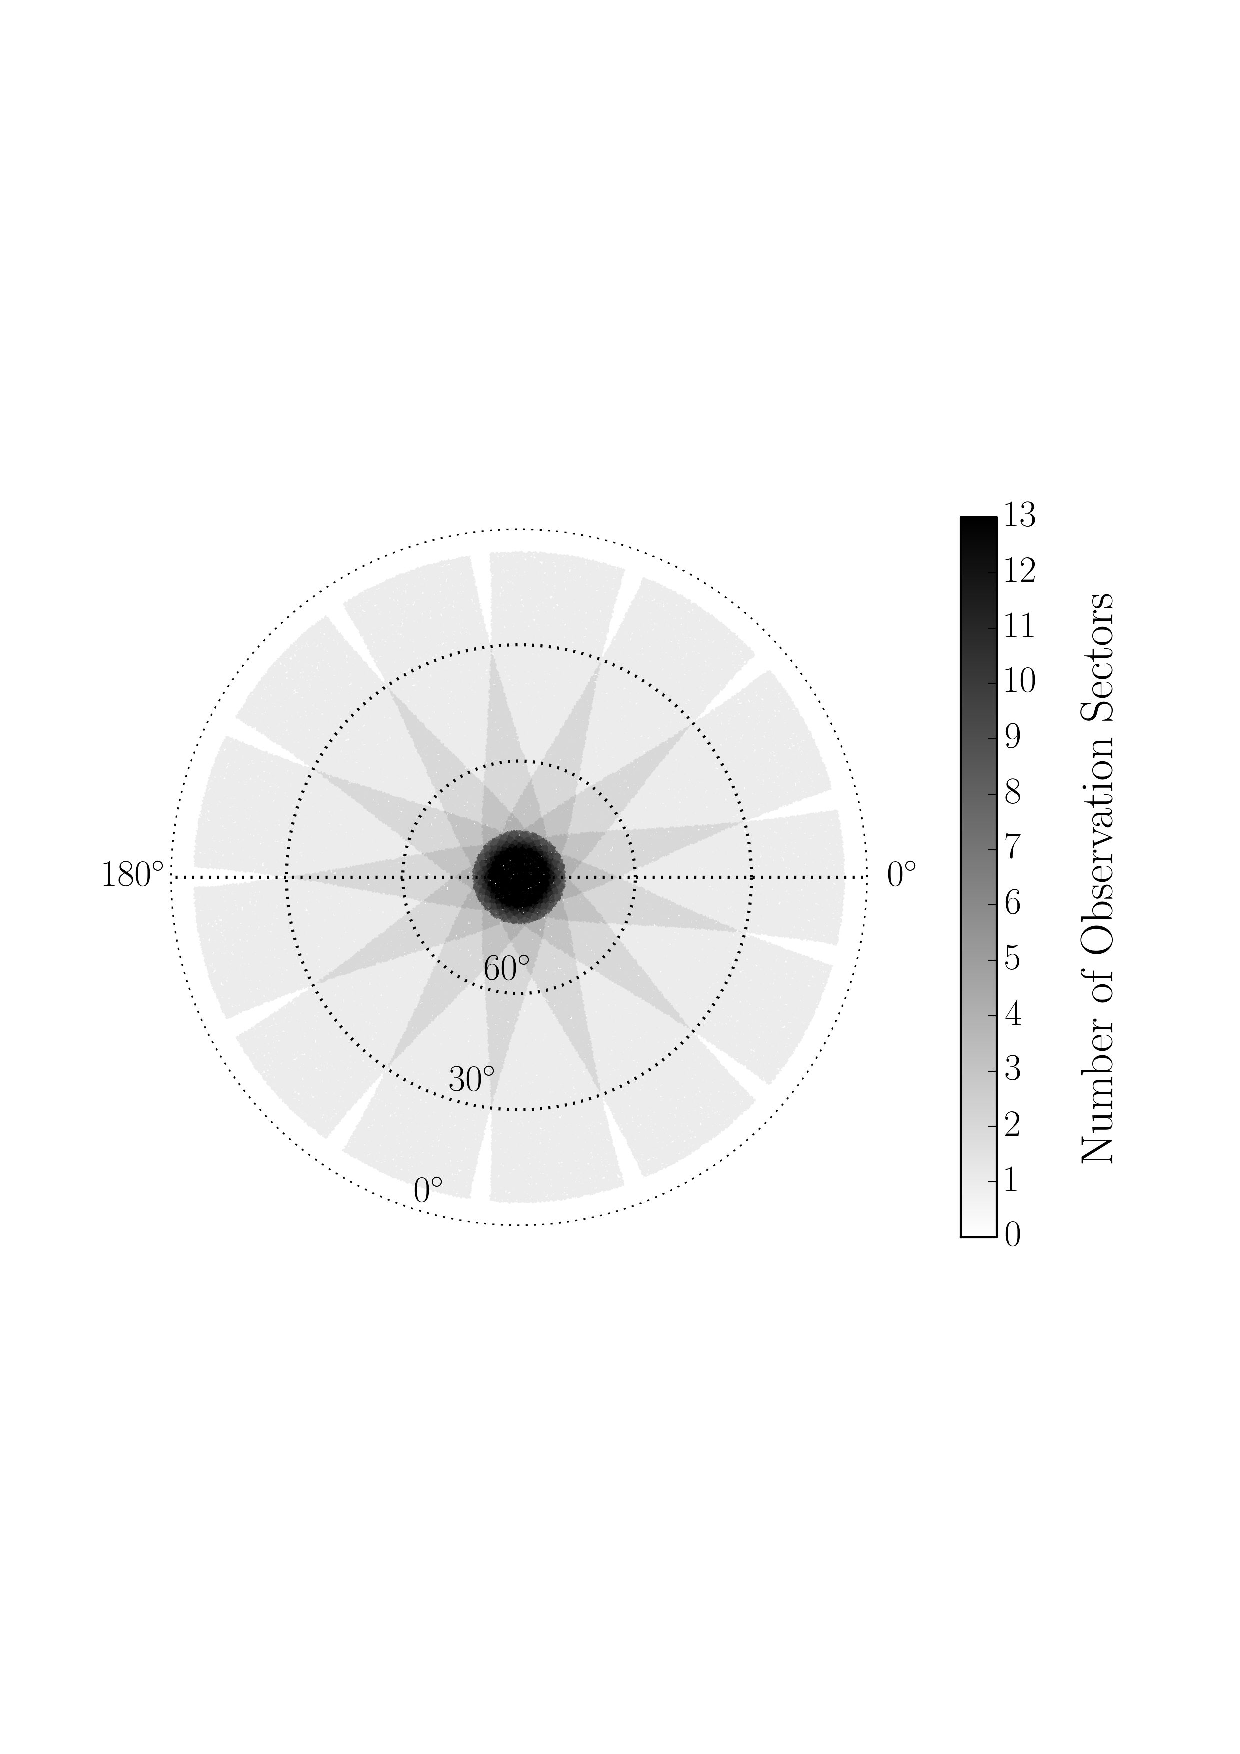
\includegraphics[scale=0.4]{cropped_TESSfield.pdf}
	\caption{TESS field of view, centred around the ecliptic pole. Each strip will be observed for 27 days before the satellite rotates. Image taken from \citet{campante_asteroseismic_2016}.}	
	\label{TESS field}
\end{figure} 

As well as reducing the dataset length, the bandpass that TESS will observe in is much redder than that of \kep, Figure \ref{bandpass}. This has the effect of reducing the amplitude of stellar signals (i.e the signal due to stellar granulation and oscillation). \citet{campante_asteroseismic_2016} found this bandpass correction to be 0.85.

\begin{figure}
	\centering
	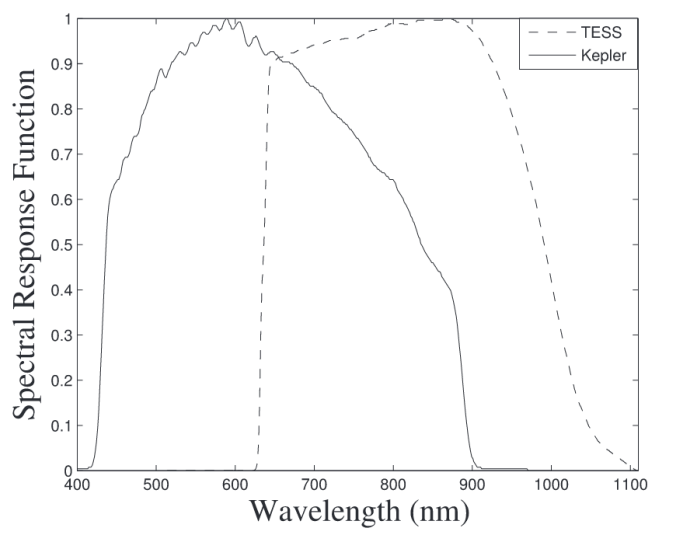
\includegraphics[scale=0.4]{bandpass.png}
	\caption{TESS field of view, centred around the ecliptic pole. Image taken from \citet{placek_combining_2016}.}	
	\label{bandpass}
\end{figure} 

Thirdly, the instrumental noise level in \kep \ is different to the noise level in TESS. The noise level for the \kep \ satellite depends on the \kep \ magnitude of the star, $K_{p}$. The noise can be calculated using
\begin{equation}
\frac{10^{6}}{c} \times \sqrt{c+9.5 \times 10^{5}\Bigg(\frac{14}{K_{p}}\Bigg)^{5}} ,
\end{equation}
where
\begin{equation}
c = 1.28 \times 10^{0.4(12-K_{p})+7} ,
\end{equation}
from \citet{chaplin_predicting_2011}.

As well as subtracting this noise from the signal, instrumental noise from TESS needed to be added. This noise was estimated using the `calc noise' IDL procedure (from William Chaplin, private communication), which depends on the $I_{c}-$band magnitude of the star and the number of pixels in the photometric aperture used when observing the star. This is given by
\begin{equation}
N_{\rm aper} = 10 \times (n+10) , 
\end{equation}
where $n$ is
\begin{equation}
n = 10^{-5.0} \times 10^{ 0.4 \times (20-I_{\rm mag})} .
\end{equation}

These three adjustments - the length of observation, the bandpass, and the noise level - were performed in the time and frequency domains. The methods used are outlined in Figures \ref{ts flowchart} and \ref{fr flowchart}.

\begin{figure}
	\centering
	\includegraphics[scale=0.3, trim={0 3cm 10cm 0}]{"TRG timeseries flowchart".pdf}
	\caption{Flow chart of the method to convert the data from \kep \ to TESS observations in the time domain.}	
	\label{ts flowchart}
\end{figure} 

\begin{figure}
	\centering
	\includegraphics[scale=0.3, trim={0 3cm 0 0}]{"TRG frequency flowchart".pdf}
	\caption{Flow chart of the method to convert the data from \kep \ to TESS observations in the frequency domain.}	
	\label{fr flowchart}
\end{figure}


\section{Detection Test}

\section{KDE}




\bibliographystyle{mnras}
\bibliography{TRG}

\bsp
\label{lastpage}
\end{document}
